%!TEX root = ../these.tex

\chapter{
  Описание формата файлов DBS
}
\label{app:dbs}

DBS ---
унаследованный двоичный формат файла
обмена информацией в CAD-системах.
В данной диссертационной работе
используется в основном представление
геометрической информации о плоских деталях.

DBS-файл состоит из произвольного количества DBS-записей.
Каждая запись имеет тип, определяющий какие данные в ней содержатся.
Основные типы записей сведены в табл.~\ref{tab:dbs.records}.

\begin{table}[h]
  \caption{Основные виды DBS-записей}
  \label{tab:dbs.records}
  \centering
  \begin{tabular}{|r|l|}
    \hline
    Тип записи & Назначение \\
    \hline
    1  & Геометрия одного контура детали  \\
    2  & Копия контура (с геометрическим преобразованием) \\
    4  & Последовательность обработки \\
    5  & Текст  \\
    7  & Плоскость  \\
    8  & Объединение нескольких контуров в деталь \\
    9  & Фаска  \\
    10 & Револьверная головка \\
    11 & Токарный инструмент  \\
    12 & Инструментальный блок  \\
    13 & Приспособление \\
    21 & Фрезерный инструмент \\
    25 & Маркировка \\
    26 & Наименование детали  \\
    27 & Площадь и периметр детали  \\
    28 & Примечание \\
    \hline
  \end{tabular}
\end{table}

Для каждой записи указывается длина,
это позволяет пропускать неизвестные или
неинтересные типы записей,
читая только необходимые в данный момент.
Благодаря этому формат DBS
легко расширяем,
возможно создание новых типов записей
без необходимости изменять существующий
код импорта / экспорта.

Служебная информация в полях записей систематически дублируется,
что усложняет задачу корректной записи DBS-файла.

\section*{Заголовок записи}

Все записи
(кроме последней)
начинаются со стандартного заголовка,
содержащего длину, тип записи
и служебную информацию.

\newcommand{\dbsRecord}[1]{
  \noindent
  \begin{tabularx}{\textwidth}{|>{\raggedleft}p{3em}|>{\centering}p{4em}|>{\centering}p{5em}|X|}
    \hline
    \multicolumn{1}{|c|}{Смещение} &
    \multicolumn{1}{c|}{Тип}      &
    \multicolumn{1}{c|}{Имя}      &
    \multicolumn{1}{c|}{Описание}     \\
    \hline
    #1
    \hline
  \end{tabularx}
}

\dbsRecord{
  +0  & int16 & $size$ & Размер записи (в 4-байтных словах) \\
  +2  & int16 & $id'$ & Не используется или копия поля $id$ \\
  +4  & int16 & $size'$ & Копия поля $size$ \\
  +6  & int16 &  &  \\
  +8  & int16 & $type$ & Тип записи (1, 2, 4, 5, \dots) \\
  +10 & int16 &  &  \\
  +12 & int16 & $id$ & Номер записи \\
  +14 & int16 &  &  \\
  +16 & ?     &  & Данные записи (зависит от типа $type$)  \\
}

Полный размер записи в байтах вычисляется по формуле
$4 \cdot (size+1)$,
что для концевой записи дало бы 0,
а для всех остальных записей дает осмысленное значение.
Теоретически возможны записи с любым неотрицательным значением поля
$size$,
но на практике
$size \geqslant 4$.

Семантика поля $id$ запутана.
В первом приближении это номер записи, что часто и бывает.
Однако, номера не обязаны идти подряд и даже возрастать,
допустимы любые неотрицательные значения.
Зачастую, например, контура деталей нумеруются с 1,
а сами детали со 100,
тогда $id$ записей могут идти вперемешку.

У разных объектов
(например, контура и детали)
$id$
не могут совпадать,
однако записи разного типа
(например, 8, 26, 27, 28),
описывающие одну деталь,
обязаны иметь одинаковый
$id$.

Допустимы ссылки вперед,
когда например, сначала описывается деталь с
$id=1$,
в которую включен контур с
$id=2$,
который размещается в файле после содержащей его детали.
Однако рекомендуется при записи файла таких ситуаций избегать
и ссылаться в каждой записи только на уже описанные
(находящиеся ближе к началу файла)
записи.

Далее приведены описания только DBS-записей,
используемых для хранения геометрической информации
о плоских деталях,
ограниченных контурами,
состоящими из отрезков прямых
и круговых дуг.

\section*{Копия контура (тип записи 2)}
Данная запись часто называется <<копией геометрии>>,
потому что ее задача ---
взять контур
(последовательность точек)
из записи типа 1 и создать его копию путем поворота / отражения и смещения.
Таким образом достигается значительное
сокращение объема файла,
поскольку типичная раскройная карта
содержит множество копий одной и той же детали,
отличающихся друг от друга только положением на листе.

\dbsRecord{
  +0  & dbs   & & Стандартный заголовок \\
  +16 & int16 & $subtype$ & Подтип записи (1, 2, 3) \\
  +18 & int16 &  &  \\
  +20 & int16 & $text$ & Признак наличия текста, связанного с контуром~(0, 1) \\
  +22 & int16 &  &  \\
  +24 & int16 & $autoseq$ & Признак наличия автопоследовательности~(0, 1) \\
  +26 & int16 &  &  \\
  +28 & int16 & $part$ & $id$ детали \\
  +30 & int16 &  &  \\
  +32 & int16 & $original$ & $id$ исходного контура \\
  +34 & int16 &  &  \\
  +36 & int16 & $rev$ & Признак реверса (-1, 0, 1, 2) \\
  +38 & int16 &  &  \\
  +40 & float32 & $\cos_{xx}$ & Матрица поворота / отражения \\
  +44 & float32 & $\sin_{xx}$ &  \\
  +48 & float32 & $\cos_{yx}$ &  \\
  +52 & float32 & $\sin_{yx}$ &  \\
  +56 & float32 & $\Delta_x$ & Смещение по горизонтали \\
  +60 & float32 & $\Delta_y$ & Смещение по вертикали   \\
}

Поле
$part$
---
отсылка к группе записей
(все с одинаковым $id$),
описывающей деталь,
в которую входит указанный контур.
Для первого
(внешнего)
контура детали
$part = -id$
детали,
для всех остальных
$part = id$.
Тем самым дублируется информация из записи 8.

Поле
$original$
содержит $id$ записи типа 1,
которая копируется.
В записи типа 1 поля $id$ и $original$ совпадают,
в записи типа 2 всегда различаются.

Если в поле
$rev \ne 0$,
значит точки контура надо обходить в обратном порядке --- от последней к первой.
При этом следует изменить знак всех полей $bulge$ в записи 1.

Геометрическое преобразование всех точек задается формулой:
\begin{equation}
  \begin{cases}
    x' = \cos_{xx} \cdot x + \cos_{yx} \cdot y + \Delta_x
    \\
    y' = \sin_{xx} \cdot x + \sin_{yx} \cdot y + \Delta_y
  \end{cases}
\end{equation}

Матрица поворота зачастую бывает единичной,
то есть копия получается из оригинала простым сдвигом.
Смещение для записей типа 1 как правило является нулевым,
а для записей 2 --- никогда.

\section*{Геометрия контура (тип записи 1)}
Данная запись часто называется <<геометрия>>,
так как содержит собственно список точек контура.
Она содержит также всю информацию из записи 2,
но здесь геометрическое преобразование как правило
тривиально
(ни сдвига, ни поворота, ни отражения).

\dbsRecord{
  +0  & rec2   & & Запись типа 2 (копия геометрии) \\
  +64 & point & $point_1$ & Первая точка контура \\
  +72 & point & $point_2$ & Вторая точка контура \\
  +84 & point & $point_3$ & Третья точка контура \\
  +96 & point & $point_i$ & \dots \\
}

Количество точек в записи явно не указано,
но легко вычисляется исходя из размера записи
(поле $size$ стандартного заголовка).

\subsection*{Точка контура}
\dbsRecord{
  +0  & float32   & $x$ & $X$-координата \\
  +4  & float32   & $y$ & $Y$-координата \\
  +8  & float32   & $bulge$ & Выпуклость участка контура \\
  +12  & point   & & Следующая точка контура \\
}

Поля
$x$ и $y$ ---
двумерные координаты точки в виде
чисел с плавающей точкой  IEEE-754
(в миллиметрах).

Поле
$bulge$ ---
кривизна участка контура от данной точки до следующей,
определяемая как
$$
bulge =
\tg \frac{\varphi}{4}
,
$$
где
$\varphi$ --- угол дуги
(или 0 для отрезка прямой).
Параметр $bulge$
последней точки никогда не используется и всегда игнорируется,
обычно там записывается $0.0$.
Знак
$bulge$
определяется направлением обхода дуги,
положительным считается обход против часовой стрелки,
что немного противоречит знаку обхода контура.

По соглашению,
материал детали при движении по контуру остаётся справа.
Таким образом, внешние контура обходятся по часовой стрелке,
внутренние --- против.

В файле нет никакого признака того,
что контур замкнут,
хотя в некоторых случаях это важно.
Определить замкнутость можно только сравнением координат первой и последней точки контура.
Обычно это сравнение делается с некоторой точностью
(например до $1\cdot 10^{-3}$),
но зачастую имеет смысл простое побитовое сравнение.

\section*{Связка контуров в деталь (тип записи 8)}
Это основная запись о детали,
Содержит список входящих в неё контуров.
Эти же сведения продублированы в их поле $part$.
Как правило эта запись сопровождается другими записями
с тем же $id$
(чаще всего 26 --- наименование и
27 --- площадь и периметр).

\dbsRecord{
  +0  & dbs   &  & Стандартный заголовок \\
  +16  & int16   & $id_1$ & $id$ первого контура \\
  +18  & int16   &  &  \\
  +20  & int16   & $id_2$ & $id$ второго контура \\
  +22  & int16   &        &  \\
  +24  &         &        & \dots \\
}

Количество контуров также никак не указано,
но вычисляется по размеру записи.

\subsection*{Обозначение детали (тип записи 26)}
Здесь указывается обозначение детали (как правило совпадает с именем файла).
Эта запись всегда идёт в паре с записью типа 8
(контура, относящиеся к детали)
с тем же самым $id$.

\dbsRecord{
  +0  & dbs   &  & Стандартный заголовок \\
  +16  & char[8]   & $partid$ & Обозначение детали \\
}

По историческим причинам обозначение детали хранится в странном формате:
\begin{itemize}
  \item
  Строка дополняется до 8 символов пробелами справа
  \item
  В каждой паре символы переставляются
\end{itemize}
Таким образом деталь с $partid$ <<CIRCLE1>>
в поле $partid$ будет иметь 8 символов
<<ICCREL 1>>.

Во время разработки формата DBS
стандарта Unicode еще не существовало,
поэтому в обозначении детали
рекомендуется использовать только
печатные ASCII-символы.

\subsection*{Измерения детали (тип записи 27)}

\dbsRecord{
  +0  & dbs   &  & Стандартный заголовок \\
  +16  & float32  & $area$ & Площадь детали, дм$^2$ \\
  +20  & float32  & $perimeter$ & Периметр детали, дм \\
}

Несмотря на то, что размеры детали указываются в миллиметрах,
площадь и периметр выражаются в дециметрах.

Для того, чтобы эта запись имела смысл,
в DBS-файле должна присутствовать запись типа 8
(контура, относящиеся к детали)
с тем же самым $id$.

\subsection*{Концевая запись}
Последняя запись в файле имеет особый формат
и показывает,
что продолжение чтения невозможно.

\dbsRecord{
  +0  & int16   & $eof$  & -1 \\
  +2  & int16   & $eof'$  & -1 \\
}

Достаточно было бы первого бита,
но принято помещать в конец DBS-файла
32~единичных бита.


% \begin{figure}
%   \centering
%   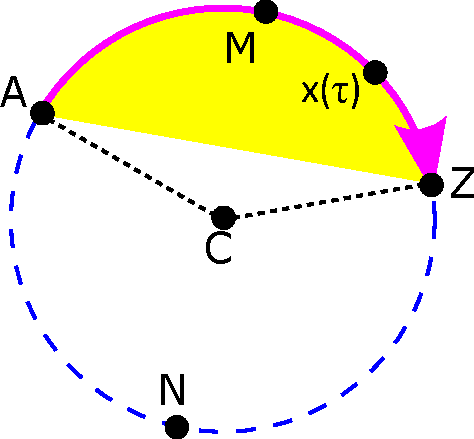
\includegraphics{arc.pdf}
%   \caption{Дуга}
%   \label{fig:app.arc}
% \end{figure}
